\section*{Introduction}
Afin de garantir une certaine qualité de code dans nos programmes, nous avons utilisé un outil de \textit{lint} (black) couplé avec le système d'\textbf{intégration continue} de GitHub. Ainsi, les développeurs étaient obligés de repasser sur leur code avant de pouvoir pousser sur une branche protégée.

De plus, nous avons suivi une logique de \textbf{développement piloté par les tests} à l'aide du package \verb|unittest| pour développer petit à petit les fonctionnalités de notre solver tout en nous assurant que nous n'avons rien cassé ailleurs.


\begin{figure}[H]
	\centering
	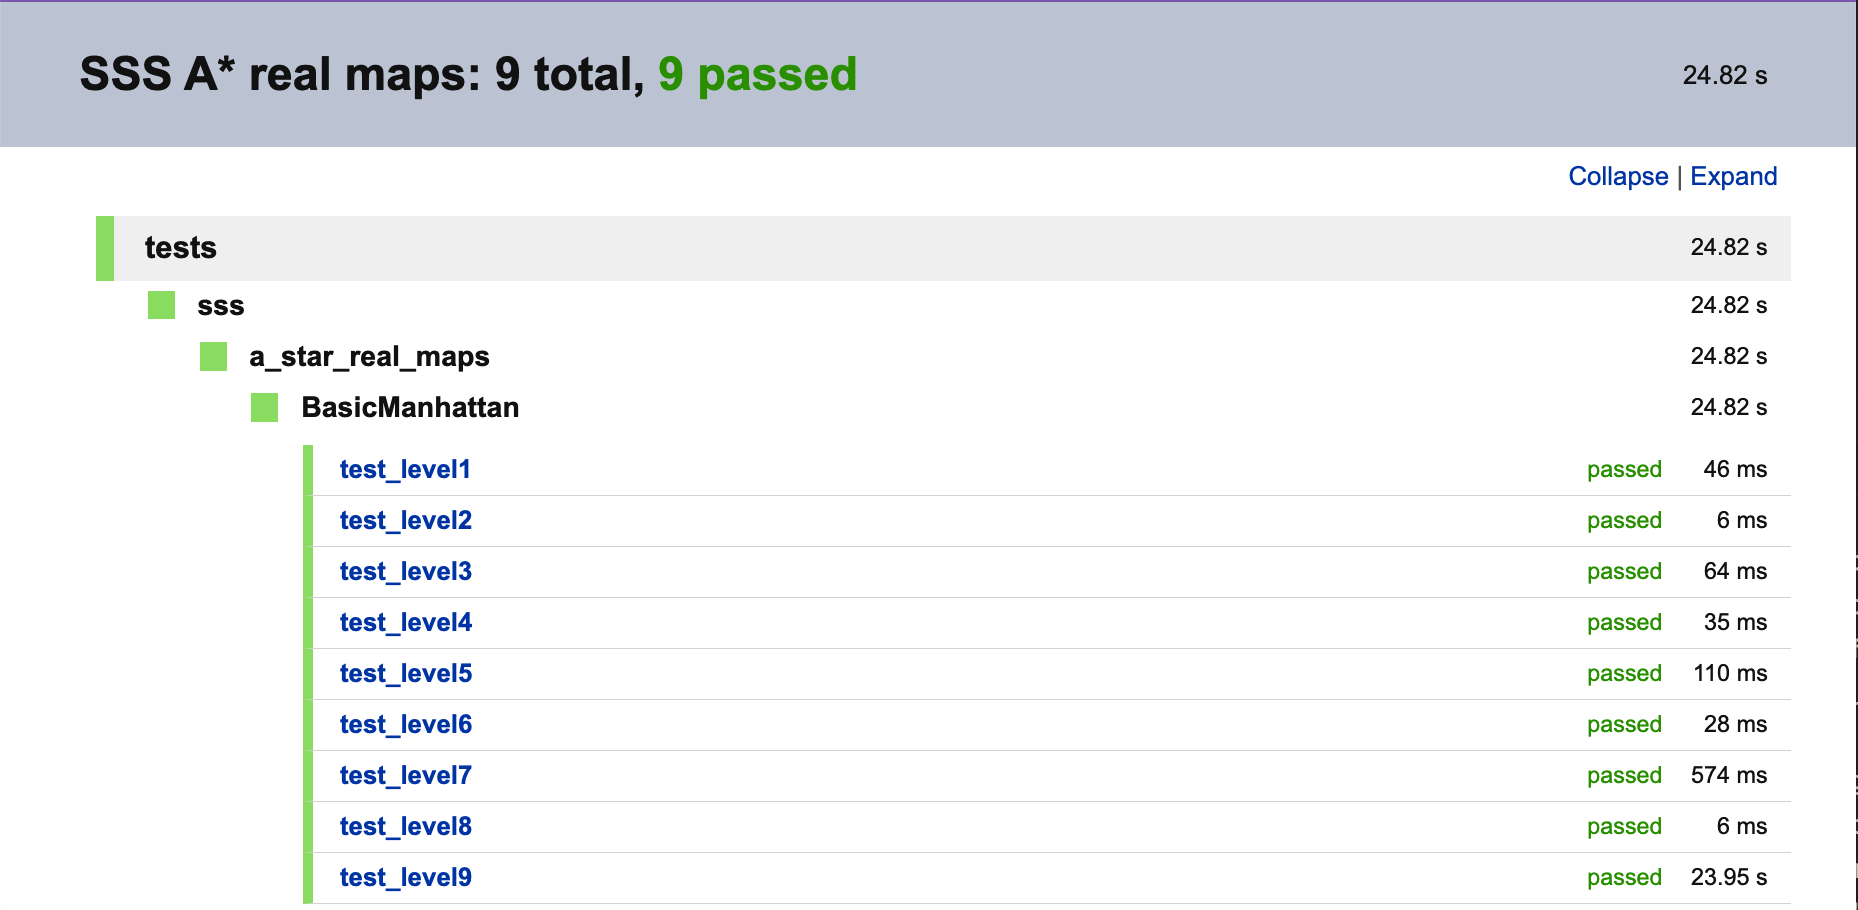
\includegraphics[height=6cm]{figures/tests_long.png}
	\caption{Sortie des tests pour la REE A*}
\end{figure}


\section{Présentation du jeu}

\subsection{Présentation des règles du jeu}

\textit{Helltaker} est un jeu vidéo freeware du style Sokoban possédant plusieurs niveaux, dans lequel le joueur doit trouver l'issue d'un labyrinthe en un nombre d'actions limité. Il s'agit d'un jeu séquentiel à un joueur.
Les objets pouvant se situer dans un niveau sont les suivants:
\begin{itemize}
	\item le héros
	\item une caisse poussable par le héros
	\item un ennemi poussable par le héros, et tuable
	\item un démon (la sortie du labyrinthe)
	\item une porte fermée
	\item une clef (permet d'ouvrir la porte)
	\item une pointe
	\item un piège (pointe ouverte un état sur deux)
\end{itemize}
Le personnage est piloté par seulement quatre touches: haut, bas, gauche, droite; effectuant des actions différentes en fonction de la position.

\begin{figure}[H]
	\centering
	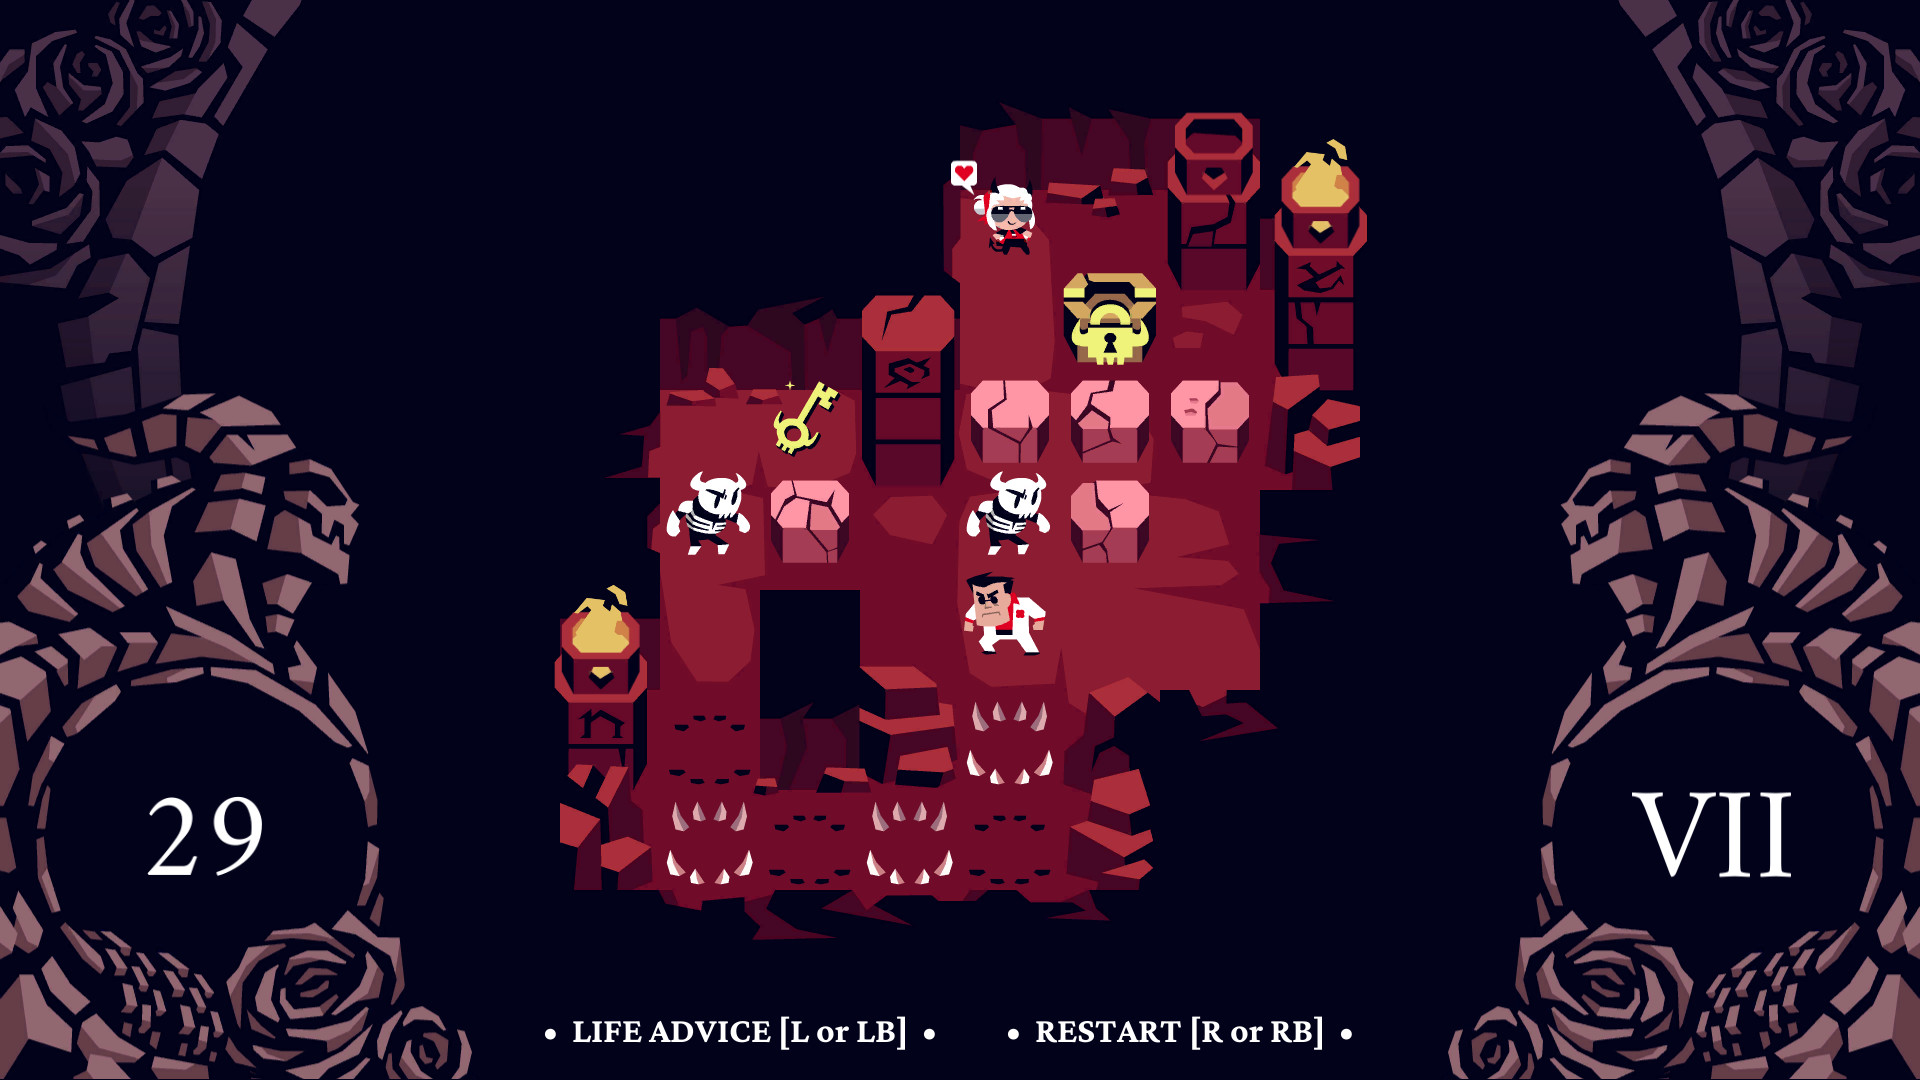
\includegraphics[height=6cm]{figures/level7.jpg}
	\caption{Niveau 7 de \textit{Helltaker}}
\end{figure}

Voici la liste des règles que nous avons considérée pour écrire nos programmes:
\begin{itemize}
	\item Le personnage peut se déplacer sur une case adjacente si elle n'est pas occupée par une caisse, un ennemi, une porte ou un démon.
	\item Le personnage peut pousser une caisse adajente si la case derrière elle n'est pas occupée par une caisse, un ennemi, une porte ou un démon.
	\item Le personnage peut pousser un ennemi adjacent si la case derrière lui n'est pas occupée par un démon.
	\item Le personnage peut donner un coup de pied dans une caisse adjacente si la case derrière elle est occupée par une caisse, un ennemi, une porte ou un démon, ce qui n'a aucun effet sur la position de la caisse ou du personnage.
	\item Un ennemi se situant sur une caisse, une porte, une pointe ou un piège actif est tué instantanément.
	\item Chaque action effectuée par le personnage réduit son compte d'actions de 1.
	\item Si le personnage se situe sur une pointe ou un piège actif après avoir effectué une action, son compte d'actions est réduit de 2 au lieu de 1.
	\item Chaque action effectuée par le personnage a pour effet d'échanger les pièges actifs et les pièges inactifs, et ce, avant le calcul de réduction du nombre d'actions.
\end{itemize}
\clearpage
\subsubsection{Représentation STRIPS}
Prédicats
\begin{lstlisting}
# un objet se situe en position P
caisse\1; ennemi\1; héros\1; clé\1; porte\1
# prédicats constants
démon\1
# définition des positions en prenant en compte les murs
gauche\2; haut\2
nombreCoups\1

\end{lstlisting}

Buts 
\begin{lstlisting}
héros(P1), démon(P2), gauche(P1, P2) 
héros(P1), démon(P2), gauche(P2, P1) 
héros(P1), démon(P2), haut(P1, P2) 
héros(P1), démon(P2), haut(P2, P1) 
\end{lstlisting}

Actions
\begin{lstlisting}
Action movement_droite(P)
    Précondition: 
    	héros(P) 
		$\wedge$ gauche(P,P1)
        $\wedge$ $\lnot$caisse(P1)
        $\wedge$ $\lnot$ennemi(P1)
        $\wedge$ $\lnot$porte(P1)
        $\wedge$ $\lnot$clé(P1)
    Postcondition: 
    	$\lnot$héros(P)
        $\wedge$ gauche(P,P1)
        $\wedge$ héros(P1)
...

Action pousser_caisse_haut(P)
	Précondition:
		héros(P)
		$\wedge$ haut()
		
		
\end{lstlisting}




\section{Recherche dans un espace d'états}
\section{Planification par SAT}

\section*{Résultats - Conclusion}